\documentclass[11pt,a4paper]{article}

% ── Packages ──────────────────────────────────────────────────────────────────
\usepackage[T1]{fontenc}
\usepackage[utf8]{inputenc}
\usepackage{newtxtext,newtxmath}
\usepackage[margin=2.4cm]{geometry}
\usepackage{microtype}
\usepackage{amsmath}
\usepackage{siunitx}
\usepackage{booktabs}
\usepackage{tabularx}
\usepackage{array}
\usepackage{graphicx}
\usepackage{caption}
\usepackage{xcolor}
\usepackage{enumitem}
\usepackage{listings}
\usepackage{tikz}
\usetikzlibrary{positioning,arrows.meta,calc}
\usepackage[numbers,sort&compress]{natbib}
\usepackage{fancyhdr}
\usepackage[colorlinks=true,linkcolor=blue!50!black,citecolor=blue!50!black,urlcolor=blue!50!black]{hyperref}
\usepackage[capitalise,noabbrev]{cleveref}

\graphicspath{{../figures/}}
\sisetup{per-mode=power,range-phrase=--,range-units=single}
\captionsetup{font=small,labelfont=bf}
\setlist{itemsep=2pt,topsep=4pt}

\definecolor{codebg}{gray}{0.96}
\lstset{basicstyle=\ttfamily\small,backgroundcolor=\color{codebg},frame=single,
  rulecolor=\color{gray!40},breaklines=true,columns=fullflexible,keepspaces=true,
  showstringspaces=false}

\pagestyle{fancy}
\fancyhf{}
\fancyhead[L]{\small Multi-model PGW for WRF with IFS/ERA5 model-level input}
\fancyhead[R]{\small Technical note}
\fancyfoot[C]{\thepage}

\newcommand{\code}[1]{\texttt{#1}}
\newcommand{\dT}{\Delta T}
\newcommand{\dRH}{\Delta \mathrm{RH}}

\title{\textbf{Multi-model pseudo-global warming perturbation of IFS/ERA5\\
model-level input for WRF}\\[4pt]
\large Technical description of \code{pgw\_workflow\_ModelLevels\_WRF}}
\author{Carlos Calvo-Sancho\\[4pt]
\small Centro de Investigaciones sobre Desertificaci\'on, Consejo Superior de Investigaciones Cient\'ificas\\
\small (CIDE, CSIC-UV-GVA), Climate, Atmosphere and Ocean Laboratory (Climatoc-Lab),\\
\small Moncada, Valencia, Spain}
\date{November 2026}

\begin{document}
\maketitle
\thispagestyle{fancy}

\begin{abstract}
\noindent
Pseudo-global warming (PGW) experiments impose a climate-change signal on the
initial and lateral boundary conditions of a regional model while the
synoptic evolution of the event is kept. This note describes a workflow that
applies monthly CMIP6 climate deltas, defined on pressure levels, directly to
the IFS/ERA5 GRIB files on 137 hybrid model levels that WPS reads to build
the initial and boundary conditions of WRF. The workflow selects $X$ CMIP6
models, from a user list or automatically, for one or more scenarios, and
produces $X+1$ perturbed sets of input files per scenario, one per model and
one for the multi-model ensemble mean (ENSMEAN). On the model levels,
temperature is shifted by the vertically interpolated delta, specific
humidity follows the change in relative humidity, and surface pressure is
adjusted until the geopotential change at \SI{300}{hPa} matches that of the
GCM. Because WPS derives the pressure of the model levels from the surface
pressure of a separate surface file, that file is perturbed consistently with
the adjusted model levels: surface and sea-level pressure, 2-m temperature
and dewpoint, and skin, sea surface and soil temperatures. A verification
step recomputes the expected change of every perturbed field. In a test case
for Hurricane Ophelia (October 2017), the errors of the 3D and surface fields
stay within the GRIB packing noise, and the geopotential constraint at
\SI{300}{hPa} is met within a few centimeters.
\end{abstract}

\tableofcontents
\newpage

% ══════════════════════════════════════════════════════════════════════════════
\section{Purpose and scope}
\label{sec:intro}

PGW experiments \citep{Schar1996,Brogli2023} compare the simulation of an
observed event with simulations driven by the same boundary conditions
perturbed with a climate-change signal $\Delta$ diagnosed from global climate
models (GCMs). In an attribution configuration, $\Delta$ is the difference
between a pre-industrial-like climate and present-day conditions. In a
projection configuration, $\Delta$ is the difference between a future and a
historical period. In both cases the design is conditional: given an event
with a similar synoptic evolution, the experiments evaluate how the imposed
thermodynamic perturbation modifies the simulated event. They do not estimate
changes in the probability of occurrence of the event or of its circulation.

This workflow is the WRF counterpart of the HARMONIE workflow
\code{pgw\_workflow\_ModelLevels}. The vertical method, the model selection,
the ENSMEAN and the verification are shared. Three aspects differ:
\begin{enumerate}
  \item The input for WPS consists of model-level files with one validity time
    each and a surface file that holds all validity times.
  \item WPS derives the pressure and height of the model levels from the
    surface pressure of the surface file (\code{calc\_ecmwf\_p}). The surface
    file is therefore perturbed with the state of the adjusted model levels of
    the same validity time (\cref{sec:surface}).
  \item The input domains of WRF are typically larger than those of HARMONIE,
    so the columns are processed in blocks to keep the memory bounded
    (\cref{sec:blocks}).
\end{enumerate}
The methodology follows PGW4ERA5 \citep{Brogli2023}.

% ══════════════════════════════════════════════════════════════════════════════
\section{Input data}
\label{sec:data}

\subsection{GRIB files for WPS}

\Cref{tab:files} lists the files of the test case, which reproduce the input
of a WRF experiment for Hurricane Ophelia. The grid is a regular
latitude--longitude grid of $401\times401$ points with \ang{0.1} spacing
(\ang{10}--\ang{50}N, \ang{60}--\ang{20}W), and the winds are
Earth-relative. The hybrid coefficients $(a, b)$ are read from the \code{pv}
array of the model-level files. WPS reads the model-level files with
\code{Vtable.ECMWF\_ml} and the surface file with an ECMWF surface Vtable,
and \code{calc\_ecmwf\_p} computes the pressure and geopotential height of
the model levels from \code{PSFC} (\code{sp}) and the hybrid coefficients.

\begin{table}[htbp]
\centering
\caption{Input GRIB files. Fields marked with $^{*}$ carry a bitmap with
missing values over land.}
\label{tab:files}
\small
\begin{tabularx}{\linewidth}{>{\raggedright\arraybackslash}p{4.6cm}Xl}
\toprule
File & Fields & Times \\
\midrule
\code{ECMWF\_PL\_YYYYMMDD\_HH.grb} & $T$, $q$, $u$, $v$ on hybrid levels 1--137;
  $\ln p_s$ and $\Phi_s$ on level 1 (GRIB2) & one per file \\
\code{ECMWF\_SFC\_*.grb} & sp, msl, 2t, 2d, 10u, 10v, skt, sst$^{*}$, ci$^{*}$,
  lsm, sd, rsn, z, stl1--4, swvl1--4 (GRIB1) & all in one file \\
\bottomrule
\end{tabularx}
\end{table}

Two properties of these files condition the design. First, the surface
pressure of the surface file (\code{sp}) and $\exp(\ln p_s)$ of the
model-level files are not identical fields. Their difference has a zero mean
but reaches \SI{650}{Pa} at some points, and the surface geopotentials of the
two files also differ. The perturbation of \code{sp} is therefore applied as
a relative change (\cref{sec:surface}). Second, ERA5 specific humidity
contains a few slightly negative values (77 points with $q$ of about
\num{-5e-8} in one of the test files), which the verification takes into
account.

\subsection{CMIP6 climate deltas and scenarios}

The deltas are monthly climatological differences on the native grid of each
GCM, with 25 pressure levels between 1000 and \SI{1}{hPa}
(\cref{tab:scen}). Attribution deltas are stored per event year (2020--2030).
With \code{ATTRIB\_YEAR=auto}, the year of the input files is used, or the
closest available year if that year is not available (2020 for Ophelia in
2017).

\begin{table}[htbp]
\centering
\caption{Scenarios available under \code{CMIP6\_deltas}.}
\label{tab:scen}
\small
\begin{tabularx}{\linewidth}{lX}
\toprule
Scenario & Delta definition \\
\midrule
\code{Attribution/ssp245/YYYY} & historical 1850--1879 minus the 30-year window
  $[\mathrm{YYYY}-15,\ \mathrm{YYYY}+14]$ (historical+ssp245), YYYY = 2020--2030 \\
\code{Future\_ssp245} & ssp245 2070--2099 minus historical 1985--2014 \\
\code{Future\_ssp370} & ssp370 2070--2099 minus historical 1985--2014 \\
\code{Future\_ssp585} & ssp585 2070--2099 minus historical 1985--2014 \\
\bottomrule
\end{tabularx}
\end{table}

% ══════════════════════════════════════════════════════════════════════════════
\section{Workflow overview}
\label{sec:overview}

A single SLURM job (\code{run\_PGW\_WRF\_ML.sh}) runs four steps
(\cref{fig:workflow}). Step~02 has two phases in a common pool of processes:
phase~A perturbs every model-level file of every member and saves the state of
its lowest model level, and phase~B perturbs the surface file of every member
with those states.

\begin{figure}[htbp]
\centering
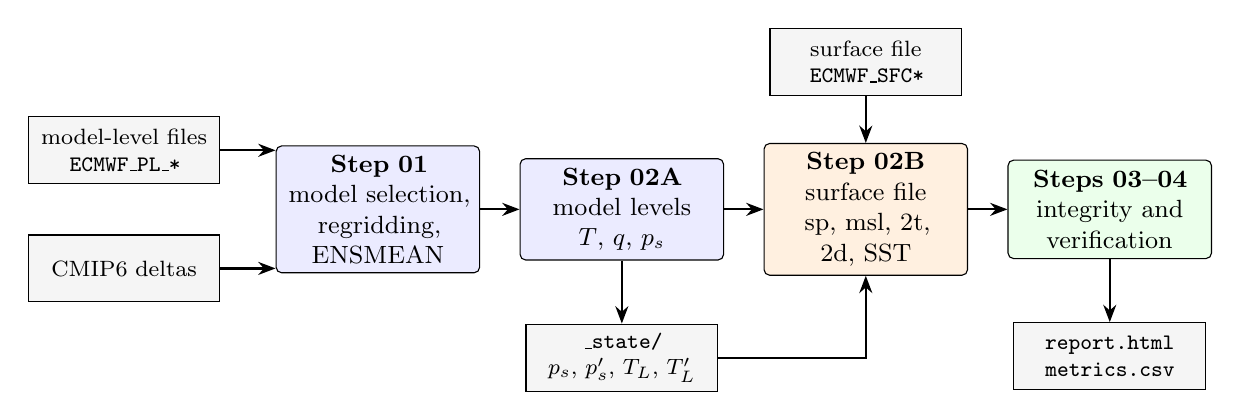
\begin{tikzpicture}[
  box/.style={draw, rounded corners=2pt, align=center, font=\small,
              minimum height=1.25cm, text width=2.35cm, fill=#1},
  box/.default=white,
  data/.style={draw, align=center, font=\footnotesize, minimum height=0.85cm,
               text width=2.2cm, fill=gray!8},
  arr/.style={-{Stealth[length=2.2mm]}, thick}]
  \node[box=blue!8] (s1) at (0,0) {\textbf{Step 01}\\model selection,\\regridding,\\ENSMEAN};
  \node[box=blue!8, right=0.5cm of s1] (sa) {\textbf{Step 02A}\\model levels\\$T$, $q$, $p_s$};
  \node[box=orange!12, right=0.5cm of sa] (sb) {\textbf{Step 02B}\\surface file\\sp, msl, 2t, 2d, SST};
  \node[box=green!8, right=0.5cm of sb] (s3) {\textbf{Steps 03--04}\\integrity and\\verification};
  \node[data, left=0.7cm of s1, yshift=0.75cm] (ml) {model-level files\\\code{ECMWF\_PL\_*}};
  \node[data, left=0.7cm of s1, yshift=-0.75cm] (cm) {CMIP6 deltas};
  \node[data, below=0.8cm of sa] (st) {\code{\_state/}\\$p_s$, $p_s'$, $T_L$, $T_L'$};
  \node[data, above=0.6cm of sb] (sf) {surface file\\\code{ECMWF\_SFC*}};
  \node[data, below=0.8cm of s3] (rep) {\code{report.html}\\\code{metrics.csv}};
  \draw[arr] (ml.east) -- (s1.west |- ml.east);
  \draw[arr] (cm.east) -- (s1.west |- cm.east);
  \draw[arr] (s1) -- (sa);
  \draw[arr] (sa) -- (sb);
  \draw[arr] (sb) -- (s3);
  \draw[arr] (sa) -- (st);
  \draw[arr] (st) -| (sb);
  \draw[arr] (sf) -- (sb);
  \draw[arr] (s3) -- (rep);
\end{tikzpicture}
\caption{Structure of the workflow. Each scenario produces $X+1$ members, and
each member is a complete set of model-level and surface files for WPS.}
\label{fig:workflow}
\end{figure}

% ══════════════════════════════════════════════════════════════════════════════
\section{Step 01: scenarios, models and deltas on the input grid}
\label{sec:step01}

\subsection{Model screening and selection}

A model is a candidate when all required variables are present (\code{ta},
\code{hur}, \code{zg}, \code{tas}, \code{ts}, \code{hurs}, plus \code{ps} with
\code{PS\_MODE=gcm} and \code{ua}, \code{va} with \code{PERTURB\_WIND=true}).
With \code{COMMON\_MODELS=true}, only models complete in every requested
scenario are kept. Models that fail any check, or fail while being read or
regridded, are excluded with a warning.

The user chooses the models as an explicit list, all candidates, or an
automatic selection of $N$ models. The automatic selection describes each
model with three features averaged over the domain box on its native grid and
over the months of the input files,
\begin{equation}
  \mathbf{x}_m = \bigl(\, \overline{\dT}_{850-300},\ \Delta T_{\mathrm{as}},\
  \overline{\dRH}_{850-500} \,\bigr),
\end{equation}
concatenated over the scenarios when the models are common. The features are
standardized, $z_{m,j} = (x_{m,j}-\mu_j)/\sigma_j$. The \code{spread} method
starts from the model closest to the multi-model mean and adds, one at a
time, the model whose minimum distance to the already selected models is
largest,
\begin{equation}
  s_{n+1} = \arg\max_{m \notin S_n}\ \min_{s \in S_n} \lVert \mathbf{z}_m - \mathbf{z}_s \rVert ,
\end{equation}
so that the $N$ models span the range of the full ensemble. The
\code{representative} method takes the $N$ models closest to the multi-model
mean.

\subsection{Horizontal interpolation and ensemble mean}

The deltas of each selected model are interpolated bilinearly to the input
grid points, after filling missing values below the GCM orography by constant
vertical extrapolation. Each variable is interpolated from its own GCM grid.
Some models store the 3D and the 2D variables on grids shifted by half a grid
cell (for example, ACCESS-ESM1-5 uses 144 latitudes for \code{ta} and 145 for
\code{tas}). Reusing the grid of the first variable for all of them misplaces
the surface deltas by up to \SI{0.6}{K}, an error that the verification of
the regridding detects (\cref{sec:verif}). The winds of the input grid are
Earth-relative, so $\Delta u$ and $\Delta v$ are not rotated.

The ENSMEAN deltas are the equal-weight mean of the regridded deltas of the
$X$ models, for every month, level and variable,
$\Delta_{\mathrm{ENS}} = X^{-1}\sum_m \Delta_m$. The ENSMEAN is applied as
one more member, so its perturbation is internally consistent.

% ══════════════════════════════════════════════════════════════════════════════
\section{Step 02A: PGW on hybrid model levels}
\label{sec:step02}

The algorithm adapts \code{step\_03\_apply\_to\_era.py} of PGW4ERA5
\citep{Brogli2023} with \code{i\_reinterp = 0} and is identical to that of the
HARMONIE workflow.

\paragraph{Hybrid coordinate and temporal selection.}
$p_{k+1/2} = a_{k+1/2} + b_{k+1/2}\, p_s$ and
$p_k = (p_{k-1/2} + p_{k+1/2})/2$ \citep{ECMWF_IFS_III}. With
\code{month=auto}, the delta at validity time $t$ is
$\Delta(t) = (1-w)\Delta_m + w\Delta_{m+1}$ with
$w = (t-t_m)/(t_{m+1}-t_m)$ between mid-month dates.

\paragraph{Vertical interpolation.}
The deltas are interpolated linearly in $\ln p$ to the original full-level
pressures, with constant extrapolation outside the GCM levels. For $\dT$ and
$\dRH$, a continuous surface anchor ties the lowest levels to $\Delta
T_{\mathrm{as}}$ and $\Delta\mathrm{RH_s}$:
\begin{equation}
  \Delta(p) = \Delta_{\mathrm{std}}(p) + \bigl[\Delta_{\mathrm{sfc}} - \Delta_{\mathrm{std}}(p_s)\bigr]
  \max\!\left(0,\ 1 - \frac{p_s - p}{D}\right),\qquad D = \SI{100}{hPa}.
  \label{eq:anchor}
\end{equation}

\paragraph{Temperature and humidity.}
$T' = T + \dT$. Relative humidity is computed with the IFS mixed-phase
saturation vapor pressure \citep{ECMWF_IFS_IV}, so that $q \to
\mathrm{RH} \to q$ is exactly invertible, and
\begin{equation}
  \mathrm{RH}' = \min\!\Bigl[\max\bigl(\mathrm{RH} + \dRH,\ 0.5\,\mathrm{RH}\bigr),\ \max(\mathrm{RH}, 1)\Bigr],
  \qquad
  q' = q + w_q(p)\,\bigl[q(\mathrm{RH}', T', p') - q\bigr],
\end{equation}
where $w_q$ decreases linearly in $\ln p$ from 1 at \SI{150}{hPa} to 0 at
\SI{100}{hPa}, so that the stratospheric specific humidity is not modified.

\paragraph{Surface pressure.}
The geopotential is integrated upward from the unchanged surface
geopotential, $\Phi_{k-1/2} = \Phi_{k+1/2} + R_d T_{v,k}
\ln(p_{k+1/2}/p_{k-1/2})$, and $p_s$ is iterated,
\begin{equation}
  E = \bigl[\Phi'(p_{\mathrm{ref}}) - \Phi(p_{\mathrm{ref}})\bigr] - g\,\Delta z_g(p_{\mathrm{ref}}),\qquad
  p_s \leftarrow p_s - 0.95\, \frac{p_s}{R_d\, T'_L}\, E,
\end{equation}
with $p_{\mathrm{ref}} = \SI{300}{hPa}$ and $q'$ recomputed at each
iteration, until $\max|E| < \SI{0.15}{m^2.s^{-2}}$. It converges in five or
six iterations in the test case.

\paragraph{Wind (optional).}
With \code{PERTURB\_WIND=true}, $u' = u + \Delta u$ and $v' = v + \Delta v$.

\paragraph{State of the lowest level.}
For every validity time, the workflow saves $p_s$, $p_s'$, $T_L$, $T_L'$,
$\Phi_s$ and, if the wind is perturbed, $\Delta u_L$ and $\Delta v_L$ of the
lowest model level to \code{<member>/\_state/}.

\subsection{Column blocks}
\label{sec:blocks}

The perturbation of a column does not depend on the other columns. The
columns are therefore processed in blocks of \code{CHUNK} columns (20\,000
by default), and the full 3D arrays kept in memory are only the original and
perturbed $T$ and $q$. For the $401\times401\times137$ test domain, the peak
memory decreases from about \SI{4}{GB} to \SI{1.9}{GB} per process, and the
results are identical to processing the whole domain at once. The default job
requests 16 processes and \SI{64}{GB}.

% ══════════════════════════════════════════════════════════════════════════════
\section{Step 02B: surface file consistent with the model levels}
\label{sec:surface}

For every validity time of the surface file with a model-level file, the
saved state of the lowest model level is used (\cref{tab:sfc}).

\begin{table}[htbp]
\centering
\caption{Perturbation of the surface file. $T_L$ is the temperature of the
lowest model level, $\Phi_s$ and $z_s = \Phi_s/g$ the surface geopotential
and height of the model-level file, $e_w$ the IFS saturation vapor pressure
over water and $T_d(e)$ its inverse.}
\label{tab:sfc}
\small
\begin{tabularx}{\linewidth}{lX}
\toprule
Field & Perturbation \\
\midrule
sp & $\mathrm{sp}' = \mathrm{sp}\cdot p_s'/p_s$ \\
msl & $\mathrm{msl}' = \mathrm{msl}\cdot\dfrac{p_s'}{p_s}\exp\!\left[\dfrac{\Phi_s}{R_d}\left(\dfrac{1}{\bar T'}-\dfrac{1}{\bar T}\right)\right]$,
  \quad $\bar T = T_L + \tfrac{1}{2}\,\gamma\, z_s$, \quad $\gamma = \SI{0.0065}{K.m^{-1}}$ \\
2t & $2t' = 2t + (T_L' - T_L)$ \\
2d & $\mathrm{RH}_2 = e_w(2d)/e_w(2t)$, \quad
  $\mathrm{RH}_2' = \min[\max(\mathrm{RH}_2+\Delta\mathrm{hurs},\ 0.5\,\mathrm{RH}_2),\ \max(\mathrm{RH}_2,1)]$, \quad
  $2d' = T_d\bigl(\mathrm{RH}_2'\, e_w(2t')\bigr)$ \\
10u, 10v & $+\Delta u_L$, $+\Delta v_L$ (only with \code{PERTURB\_WIND=true}) \\
skt, sst & $+\Delta T_s$, with an open-sea $\Delta T_s$ over the sea (eroded
  sea mask, inverse-distance filling, Gaussian smoothing) \\
stl1--4 & $+\overline{\Delta T_s} + e^{-z/2.8\,\mathrm{m}}\,(\Delta T_s - \overline{\Delta T_s})$ \\
swvl1--4, sd, rsn, ci, lsm, z & unchanged \\
\bottomrule
\end{tabularx}
\end{table}

The surface pressure follows the relative change of the adjusted $p_s$
because \code{sp} and $\exp(\ln p_s)$ are different fields in the input. The
sea-level pressure is rescaled with the hydrostatic reduction of a column
with the standard lapse rate between the surface and sea level. Over the sea
($z_s \approx 0$), $\mathrm{msl}'/\mathrm{msl} = \mathrm{sp}'/\mathrm{sp}$.
The 2-m temperature receives the $\dT$ of the lowest model level, which the
surface anchor (\cref{eq:anchor}) ties to $\Delta T_{\mathrm{as}}$, and the
2-m dewpoint keeps the 2-m relative humidity plus $\Delta\mathrm{hurs}$, with
the same bounds as in 3D.

Times of the surface file without a model-level file keep sp and msl
unchanged and use $\Delta T_{\mathrm{as}}$ for 2t. They are reported as
warnings in the log and in the report. In the Ophelia input, the surface file
has 24 times and the model-level files cover 21, so the last three times
(12 October at 06, 12 and 18~UTC) are uncoupled. WPS does not use them when
the simulation ends at 00~UTC on 12 October.

% ══════════════════════════════════════════════════════════════════════════════
\section{Steps 03 and 04: verification}
\label{sec:verif}

Step~03 checks the integrity of each member: number of messages, metadata,
bit-identical values of every non-perturbed field, finite values, SST
bitmaps of every time and the absence of new negative values of $q$ beyond
one packing unit.

Step~04 recomputes the expected change of every perturbed field and compares
it with the difference between the PGW and the original files, for every
model-level file and the matching time of the surface file. GRIB encoding
quantizes each value with a step $u = 2^{E}\,10^{-D}$, the packing unit
(p.u.). For sp, msl, 2t and 2d, the expected value depends on other packed
fields ($\ln p_s'$, $T_L$, $2t'$), so the tolerance adds the error propagated
from those fields to the rounding of the field itself (\cref{tab:checks}).
The statistics are accumulated over the column blocks.

\begin{table}[htbp]
\centering
\caption{Checks of Step~04.}
\label{tab:checks}
\small
\begin{tabularx}{\linewidth}{lXl}
\toprule
Check & Comparison & Tolerance \\
\midrule
Replica of $T$, $q$, skt, sst, stl1--4 ($u$, $v$) & written change minus
  recomputed change & $\le$ \SI{1}{p.u.} \\
Replica of sp, msl, 2t, 2d (10u, 10v) & written field minus recomputed field &
  rounding + propagated error \\
$\dT$ on sample columns & 300 columns with an independent interpolation & $\le$ \SI{e-3}{K} + packing \\
$\Delta z_g(p_{\mathrm{ref}})$ & reached minus GCM target & max $\le$ \SI{0.25}{m} \\
$\dRH$ (troposphere), $\mathrm{RH}_2$ & reached minus target, outside bounded points & RMSE $\le$ 0.5\% \\
Stratospheric $q$ & change above \SI{100}{hPa} & $\le$ \SI{1}{p.u.} \\
New negative $q$ & $q' < -u$ where $q \ge 0$ & none \\
Regridding & deltas on the grid minus \code{xarray.interp} of the native deltas & $\le$ \SI{0.02}{K} \\
ENSMEAN & deltas and applied $\dT$ minus the means of the models & $\le 10^{-4}$, $\le$ \SI{0.01}{K} \\
\bottomrule
\end{tabularx}
\end{table}

The criterion for negative $q$ accounts for the encoding. Where the minimum
of a level is negative, the reference value of the GRIB message is negative,
and values of about \num{1e-8} can be rounded to that reference value
(about \num{-4e-8}, or 0.35 packing units in the test files). The PGW
perturbation itself cannot produce $q' < 0$ from $q \ge 0$, because
$\mathrm{RH}' \ge 0.5\,\mathrm{RH}$.

The domain-mean relative change of $q$ is computed as a ratio of sums,
$100\sum(q'-q)/\sum q$, per level. The mean of the point ratios is dominated
by the few points with $q \approx 0$ or $q < 0$.

% ══════════════════════════════════════════════════════════════════════════════
\section{Example: Hurricane Ophelia, 7 October 2017}
\label{sec:example}

\subsection{Configuration}

The example perturbs the ERA5 input of a WRF experiment for Hurricane Ophelia
on the $401\times401$ grid of \cref{sec:data}: the model-level files valid at
00 and 06~UTC on 7 October 2017 and the surface file with its 24 times. The
job ran through SLURM with the default options of \cref{tab:opts},
\code{month=auto}, eight processes and \SI{32}{GB}, and took 13.5 minutes for
the four steps. The attribution deltas of 2020, the closest available year to
the event, and the ssp585 deltas were used, with $N=5$ common models selected
automatically with the \code{spread} method.

\subsection{Model selection}

Of 30 models complete in both scenarios, the selection returns ACCESS-ESM1-5
(the closest to the multi-model mean), EC-Earth3-Veg, GISS-E2-2-G, CanESM5
and HadGEM3-GC31-LL. In the ssp585 scenario, the tropospheric $\dT$ of the
five models (850--\SI{300}{hPa}) ranges from \SI{3.95}{K} (GISS-E2-2-G) to
\SI{7.40}{K} (CanESM5), against \SI{3.17}{K} to \SI{7.55}{K} for the 30
candidates, and their $\dRH$ between 850 and \SI{500}{hPa} ranges from
$-4.88$ (HadGEM3-GC31-LL, the lowest value of all candidates) to $+1.18$
percentage points (\cref{fig:selection}). The mean of the five models differs
from the mean of the 30 candidates by $+0.39$~K in tropospheric $\dT$ and by
$-0.72$ percentage points in $\dRH$ in ssp585, and by $-0.03$~K and $+0.03$
percentage points in the attribution scenario.

\begin{figure}[htbp]
\centering
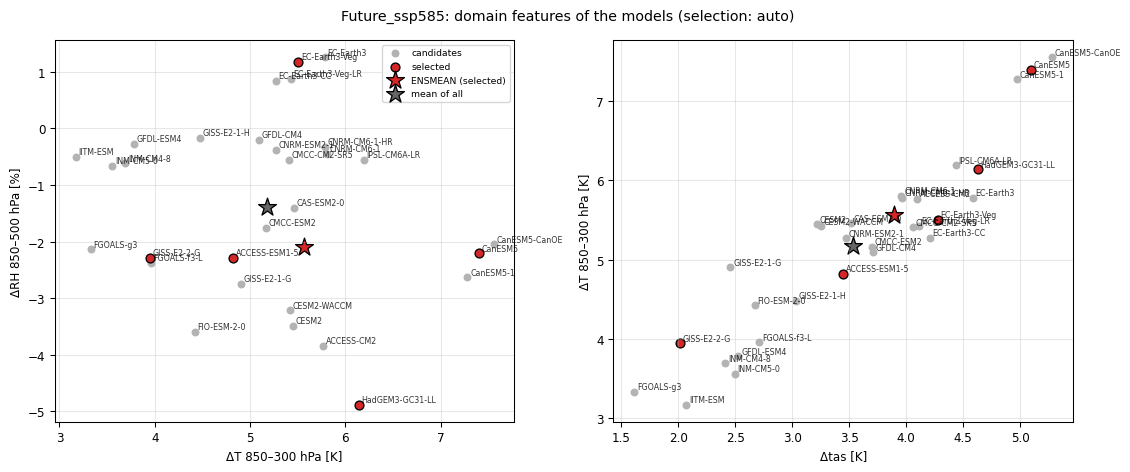
\includegraphics[width=\linewidth]{selection_Future_ssp585.png}
\caption{Domain features of the 30 candidate models in the ssp585 scenario
over the Ophelia domain (October): (left) mean $\dRH$ between 850 and
\SI{500}{hPa} against mean $\dT$ between 850 and \SI{300}{hPa}, and (right)
mean $\dT$ between 850 and \SI{300}{hPa} against $\Delta T_{\mathrm{as}}$.
Gray dots are the candidates, red dots the five models selected with the
\code{spread} method on the concatenated features of both scenarios, the red
star their mean (ENSMEAN) and the gray star the mean of all candidates.}
\label{fig:selection}
\end{figure}

\subsection{Applied perturbation}

\Cref{tab:example} lists the domain means of the applied changes. In the
ssp585 scenario, the ENSMEAN warms the domain by \SI{4.82}{K} at
\SI{850}{hPa} and \SI{5.61}{K} at \SI{500}{hPa}, with model values between
$+3.28$ and \SI{+6.07}{K} at \SI{850}{hPa}. In the attribution scenario, the
ENSMEAN cools the domain by \SI{1.52}{K} at \SI{850}{hPa}, with model values
between $-0.35$ and \SI{-2.17}{K}. The intermodel standard deviation of $\dT$
at the lowest model level ranges between 0.17 and \SI{4.41}{K} across the
domain in ssp585, with the largest values in the northwestern corner, and
between 0.26 and \SI{1.58}{K} in the attribution scenario (\cref{fig:maps}).
Specific humidity at \SI{850}{hPa} (ratio of domain means) increases by
30.0\% in the ssp585 ENSMEAN and decreases by 8.3\% in the attribution
ENSMEAN at 00~UTC, which corresponds to 6.2 and 5.5\% per kelvin of the
domain-mean $\dT$ at that level (\cref{fig:profiles,fig:scenarios}). The
surface pressure adjustment converged in five or six iterations for every
member and file.

\begin{table}[htbp]
\centering
\caption{Domain-mean applied changes for each member (mean of the files
valid at 00 and 06~UTC on 7 October 2017). $\dT$ and $\dRH$ are evaluated at
the model level closest to each pressure level. $\Delta$SST is the mean over
valid sea points of the surface file.}
\label{tab:example}
\small
\begin{tabular}{llrrrrr}
\toprule
Scenario & Member & $\dT_{850}$ (K) & $\dT_{500}$ (K) & $\dRH_{850}$ (\%) & $\Delta p_s$ (Pa) & $\Delta$SST (K) \\
\midrule
Attribution (2020) & ACCESS-ESM1-5   & $-1.36$ & $-1.65$ & $+0.28$ & $+41.3$ & $-1.02$ \\
                   & EC-Earth3-Veg   & $-2.17$ & $-2.56$ & $-1.53$ & $+26.0$ & $-1.92$ \\
                   & GISS-E2-2-G     & $-0.35$ & $-0.54$ & $+1.28$ & $-17.5$ & $-0.03$ \\
                   & CanESM5         & $-2.12$ & $-2.61$ & $+0.52$ & $-59.7$ & $-1.44$ \\
                   & HadGEM3-GC31-LL & $-1.58$ & $-1.45$ & $+2.44$ & $-38.6$ & $-1.10$ \\
                   & \textbf{ENSMEAN} & $\mathbf{-1.52}$ & $\mathbf{-1.76}$ & $\mathbf{+0.61}$ & $\mathbf{-9.4}$ & $\mathbf{-1.10}$ \\
\midrule
ssp585             & ACCESS-ESM1-5   & $+4.18$ & $+4.92$ & $-2.24$ & $+39.3$ & $+3.34$ \\
                   & EC-Earth3-Veg   & $+4.68$ & $+5.50$ & $+1.36$ & $+42.7$ & $+4.26$ \\
                   & GISS-E2-2-G     & $+3.28$ & $+4.09$ & $-3.53$ & $+14.0$ & $+1.69$ \\
                   & CanESM5         & $+6.07$ & $+7.64$ & $+0.11$ & $-68.1$ & $+5.18$ \\
                   & HadGEM3-GC31-LL & $+5.92$ & $+5.91$ & $-7.54$ & $+53.4$ & $+4.61$ \\
                   & \textbf{ENSMEAN} & $\mathbf{+4.82}$ & $\mathbf{+5.61}$ & $\mathbf{-2.35}$ & $\mathbf{+17.0}$ & $\mathbf{+3.82}$ \\
\bottomrule
\end{tabular}
\end{table}

\begin{figure}[htbp]
\centering
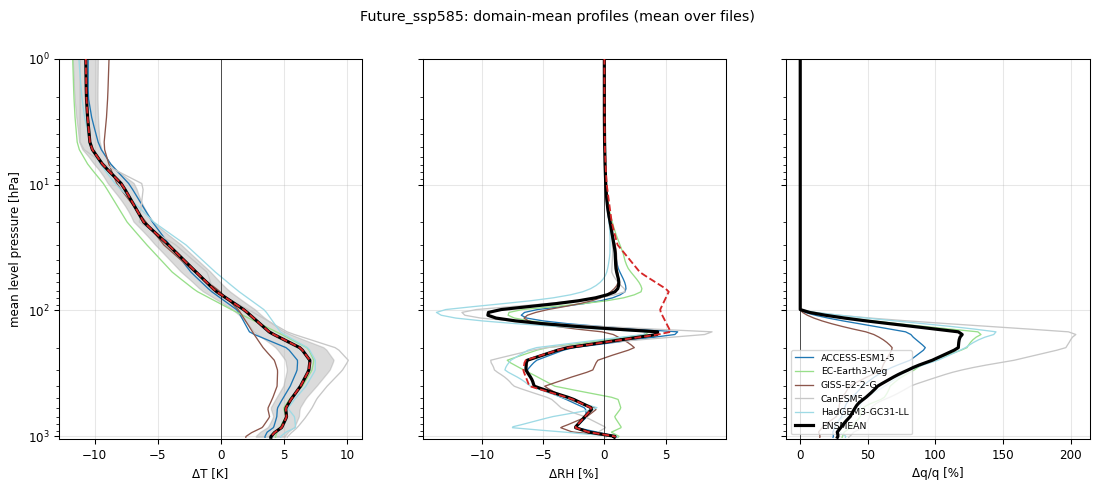
\includegraphics[width=\linewidth]{profiles_Future_ssp585.png}
\caption{Domain-mean profiles of the applied changes in the ssp585 scenario
over the Ophelia domain: (left) $\dT$, (center) $\dRH$ and (right) relative
change in specific humidity (ratio of domain means), against the mean
pressure of each model level. Thin colored lines are the five models, the
thick black line is the ENSMEAN and the gray band is $\pm1$ intermodel
standard deviation of $\dT$. Dashed red lines are the expected $\dT$ and the
unbounded target $\dRH$ of the ENSMEAN.}
\label{fig:profiles}
\end{figure}

\begin{figure}[htbp]
\centering
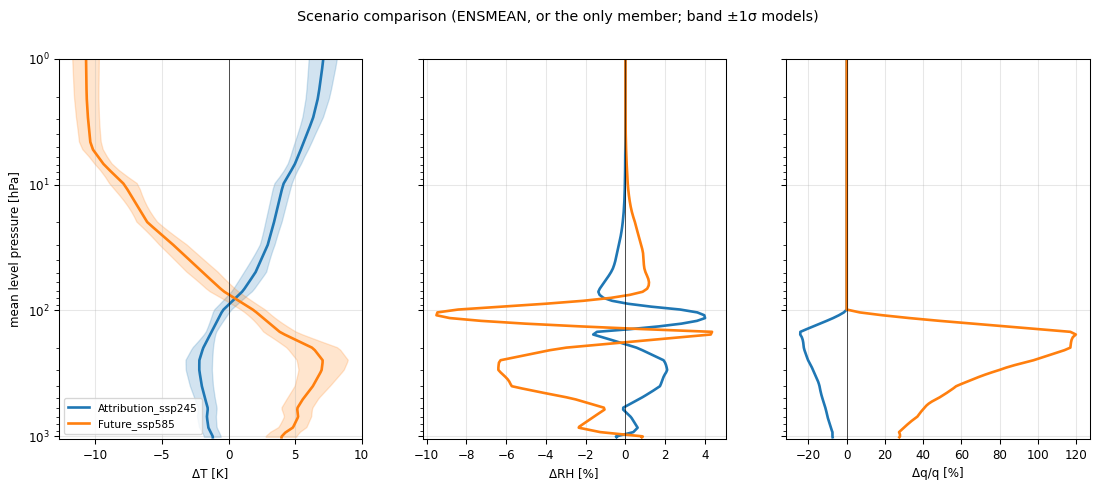
\includegraphics[width=0.85\linewidth]{scenarios.png}
\caption{ENSMEAN profiles of (left) $\dT$, (center) $\dRH$ and (right)
relative change in specific humidity for the attribution (blue) and ssp585
(orange) scenarios. Shading shows $\pm1$ intermodel standard deviation of
$\dT$.}
\label{fig:scenarios}
\end{figure}

\begin{figure}[htbp]
\centering
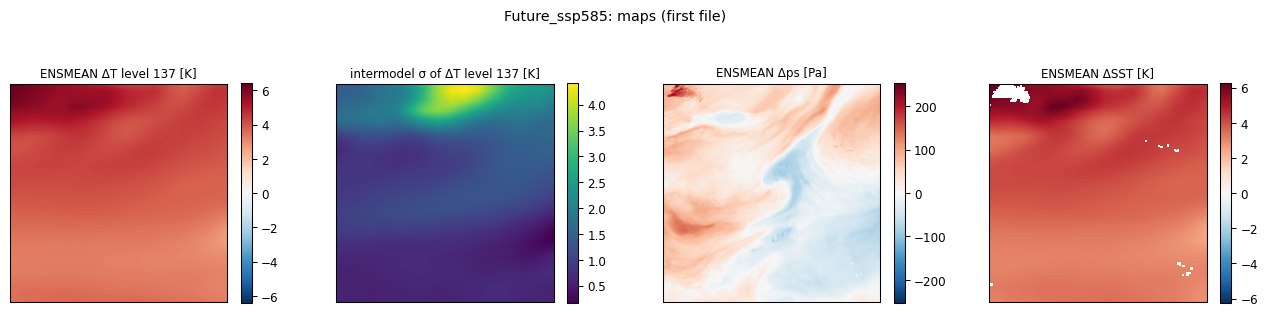
\includegraphics[width=\linewidth]{maps_Future_ssp585.png}
\caption{Maps for the ssp585 scenario at 00~UTC on 7 October 2017: (from left
to right) ENSMEAN $\dT$ at the lowest model level, intermodel standard
deviation of that $\dT$, ENSMEAN $\Delta p_s$ and ENSMEAN $\Delta$SST (land
points masked). Axes are the grid indices, with north at the top.}
\label{fig:maps}
\end{figure}

\subsection{Surface file}

At 00~UTC on 7 October, the ssp585 ENSMEAN changes the domain means of sp by
\SI{+16.3}{Pa}, msl by \SI{+15.9}{Pa}, 2t by \SI{+3.98}{K}, 2d by
\SI{+4.03}{K} and SST by \SI{+3.82}{K} (\cref{fig:sfc}). Over the ocean, the
change in msl follows that of sp, as the reduction to sea level implies for
$z_s \approx 0$. The 2-m dewpoint rises slightly more than the 2-m
temperature because the 2-m relative humidity changes only by
$\Delta\mathrm{hurs}$. In the attribution scenario, the corresponding changes
are \SI{-9.1}{Pa}, \SI{-8.9}{Pa}, \SI{-1.19}{K}, \SI{-1.24}{K} and
\SI{-1.10}{K}.

\begin{figure}[htbp]
\centering
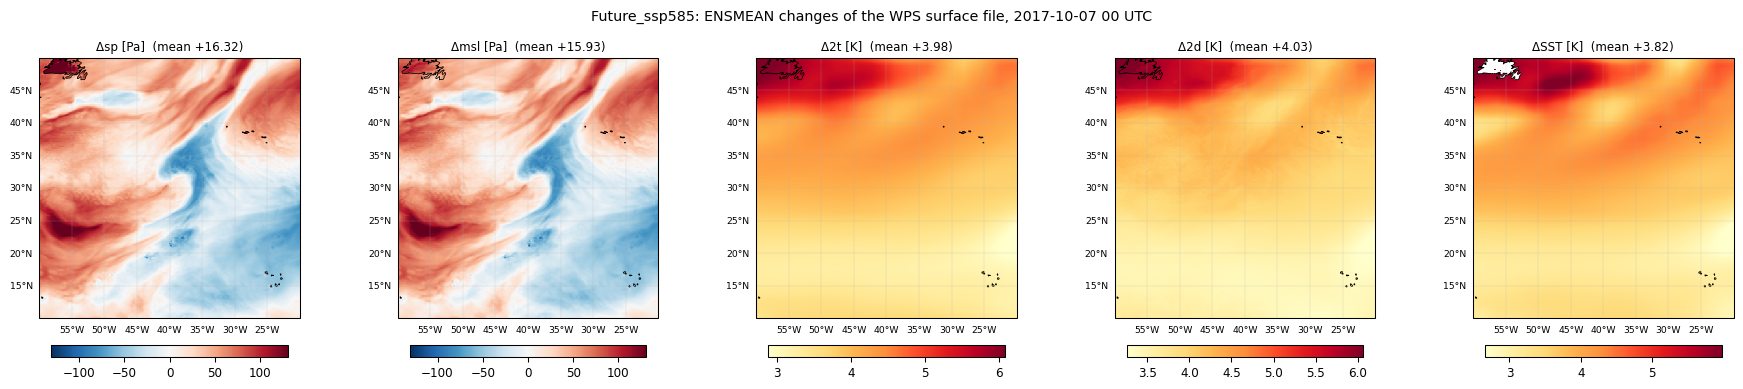
\includegraphics[width=\linewidth]{surface_Future_ssp585_ENSMEAN.png}
\caption{ENSMEAN changes of the WPS surface file for ssp585 at 00~UTC on
7 October 2017: (from left to right) sp, msl, 2-m temperature, 2-m dewpoint
and SST (land points masked). The domain mean of each field is given in the
panel title. $\Delta$sp and $\Delta$msl share the same color scale.}
\label{fig:sfc}
\end{figure}

\subsection{Verification}

All checks of \cref{tab:checks} pass for the 12 members and the two times.
The exact replicas of $T$, skt, sst and stl1--4 have maximum errors of
\SI{0.50}{p.u.}, the rounding limit of the encoding (\SI{4.9e-4}{K} for
$T$), and the replica of $q$ reaches \SI{0.57}{p.u.} The recomputed sp and
msl differ from the written fields by at most 0.22 and \SI{0.13}{Pa}, and 2t
and 2d by at most \SI{4.6e-4}{K} and \SI{4.9e-4}{K}, all within their
tolerances. The geopotential height change at \SI{300}{hPa} departs from the
GCM target by at most \SI{2.4}{cm}. The reached $\dRH$ in the troposphere and
the reached 2-m relative humidity depart from their targets by RMSEs of
0.0014 and 0.0010\%. The regridded deltas agree with \code{xarray.interp} of
the native fields within \SI{5e-7}{K} for every model, ACCESS-ESM1-5
included, and the applied $\dT$ of the ENSMEAN equals the mean applied
$\dT$ of the models within \SI{6.8e-4}{K}. Because this test uses only two
model-level files, 22 of the 24 surface times (all except 00 and 06~UTC on
7 October) are reported as uncoupled. With the complete input, only the three
times after 00~UTC on 12 October are.

\begin{figure}[htbp]
\centering
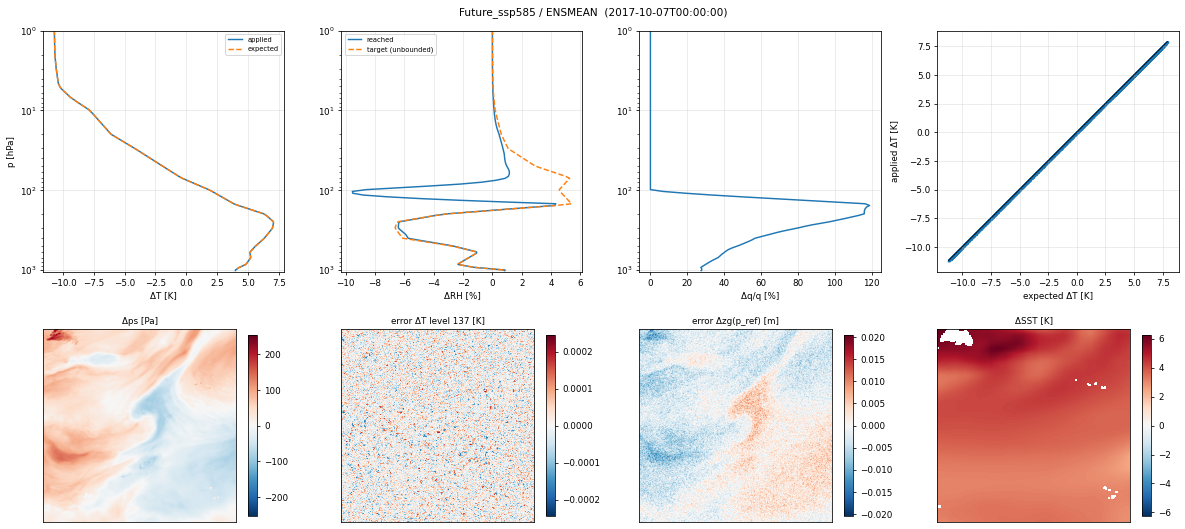
\includegraphics[width=\linewidth]{member_Future_ssp585_ENSMEAN.png}
\caption{Verification of the ssp585 ENSMEAN member at 00~UTC on 7 October
2017. Top row: domain-mean applied and expected $\dT$, reached and target
$\dRH$, relative change in specific humidity, and applied against expected
$\dT$ on 300 columns and 137 levels. Bottom row: $\Delta p_s$, error of $\dT$
at the lowest model level, error of $\Delta z_g$ at \SI{300}{hPa}, and
$\Delta$SST.}
\label{fig:member}
\end{figure}

\begin{figure}[htbp]
\centering
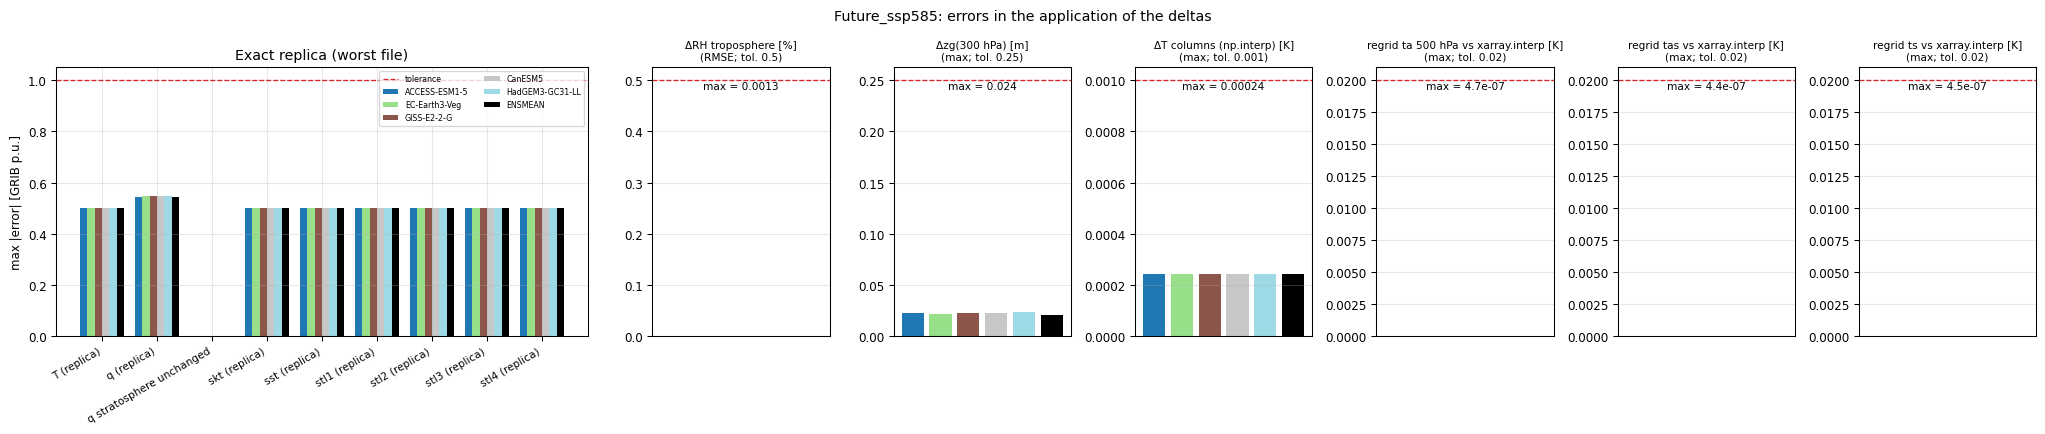
\includegraphics[width=\linewidth]{errors_Future_ssp585.png}
\caption{Worst error per member and check in the ssp585 scenario. Left: exact
replicas in GRIB packing units. Right panels: physical and independent checks
in their own units. Dashed red lines mark the tolerances of
\cref{tab:checks}.}
\label{fig:errors}
\end{figure}

\clearpage

% ══════════════════════════════════════════════════════════════════════════════
\section{Usage}
\label{sec:usage}

The options are set at the top of \code{run\_PGW\_WRF\_ML.sh}
(\cref{tab:opts}), and the job is submitted with
\begin{lstlisting}[language=bash]
sbatch run_PGW_WRF_ML.sh <path_input> <path_output> <cmip_root> <month>

# example
sbatch run_PGW_WRF_ML.sh \
    /perm/spcc/WRF_HAILCAST/input/Ophelia500m/conditions \
    /ec/res4/scratch/ecme2143/PGW_Ophelia500m \
    /ec/res4/hpcperm/ecme2143/CMIP6_deltas auto
\end{lstlisting}
WPS is then run as usual (ungrib of the model-level and surface files,
\code{calc\_ecmwf\_p}, metgrid) with the input path pointing to
\code{<path\_output>/<SCENARIO>/<MEMBER>/}. The perturbed files keep the
names, the number and order of messages and the metadata of the originals, so
the same Vtables and \code{ecmwf\_coeffs} apply. The output tree is
\begin{lstlisting}
<path_output>/
  _deltas/members.json, members.txt
  _deltas/<SCENARIO>/<MODEL|ENSMEAN>/deltas_on_grid.nc
  <SCENARIO>/<MEMBER>/ECMWF_PL_*.grb, ECMWF_SFC_*.grb   (PGW files)
  <SCENARIO>/<MEMBER>/_state/, pgw_options.json, pgw_diagnostics.jsonl
  verification/report.html, metrics.csv, summary.txt, figs/
\end{lstlisting}

\begin{table}[htbp]
\centering
\caption{Main options of \code{run\_PGW\_WRF\_ML.sh}.}
\label{tab:opts}
\small
\begin{tabularx}{\linewidth}{>{\raggedright\arraybackslash}p{4.6cm}>{\raggedright\arraybackslash}p{3.6cm}X}
\toprule
Option & Default & Meaning \\
\midrule
\code{SCENARIOS} & \code{Attribution\_ssp245} \code{Future\_ssp585} & scenarios, or \code{all} \\
\code{ATTRIB\_YEAR} & \code{auto} & event year (closest available) \\
\code{MODELS}, \code{N\_MODELS} & \code{auto}, 5 & list, \code{all} or \code{auto} \\
\code{AUTO\_METHOD} & \code{spread} & or \code{representative} \\
\code{COMMON\_MODELS}, \code{MAKE\_ENSMEAN} & \code{true}, \code{true} & common models, ENSMEAN \\
\code{ML\_PATTERN} & \code{ECMWF\_PL\_*.grb} & model-level files \\
\code{SFC\_PATTERN} & \code{ECMWF\_SFC*.grb} & surface files \\
\code{CHUNK}, \code{NPROC} & 20000, SLURM CPUs & memory control \\
\midrule
\code{PERTURB\_T}, \code{PERTURB\_Q} & \code{true} & temperature and humidity \\
\code{PERTURB\_WIND} & \code{false} & $u$, $v$, 10u, 10v \\
\code{PS\_MODE}, \code{P\_REF} & \code{hydrostatic}, \SI{30000}{Pa} & $p_s$ adjustment \\
\code{PERTURB\_MSL} & \code{true} & hydrostatic rescaling of msl \\
\code{SFC\_ANCHOR}, \code{SFC\_BLEND\_DEPTH} & \code{true}, \SI{10000}{Pa} & surface anchor \\
\code{Q\_TAPER\_BOTTOM/TOP} & 15000/\SI{10000}{Pa} & stratospheric taper of $\Delta q$ \\
\code{RH\_MIN\_FACTOR} & 0.5 & lower bound of $\mathrm{RH}'$ and $\mathrm{RH}_2'$ \\
\code{PERTURB\_SKT/SST/SOIL} & \code{true} & surface and soil temperatures \\
\bottomrule
\end{tabularx}
\end{table}

% ══════════════════════════════════════════════════════════════════════════════
\section{Limitations}
\label{sec:limits}

\begin{itemize}
  \item The experiments keep the synoptic evolution of the driving analysis
    and evaluate conditional changes in the simulated event, not changes in
    its probability, frequency or circulation. The wind is not perturbed by
    default, so similar winds in the perturbed simulations reflect the design.
  \item The deltas are monthly climatological differences. Sub-monthly
    variability of the climate signal is not represented.
  \item The selected models sample part of the intermodel uncertainty of
    $\Delta$, and the ENSMEAN of the $X$ models can differ from the mean of
    all candidates. Internal variability is not sampled.
  \item The attribution deltas exist for event years 2020--2030. Events
    outside that range use the closest year, whose present-day window differs
    from the one centered on the event.
  \item The sea-level pressure is rescaled with a standard-lapse-rate
    reduction anchored on the original msl. It is consistent with the changes
    in $p_s$ and $T_L$ but is not the IFS sea-level reduction itself.
  \item Soil moisture, snow and sea ice are not perturbed.
  \item The perturbed files have not yet been processed by WPS and integrated
    with WRF.
\end{itemize}

\section*{Code availability}
The workflow is written in Python (numpy, scipy, xarray, eccodes, matplotlib)
and Bash and is released under the MIT license at
\url{https://github.com/ccalvosa/pgw_workflow_ModelLevels_WRF}. The
repository includes a round-trip test that applies zero deltas to a
model-level and a surface file and checks that the output reproduces the
input within one packing unit.

\begin{thebibliography}{9}
\bibitem[Brogli et al.(2023)]{Brogli2023}
Brogli, R., Heim, C., Mensch, J., S{\o}rland, S.~L., and Sch{\"a}r, C.:
The pseudo-global-warming (PGW) approach: methodology, software package
PGW4ERA5 v1.1, validation, and sensitivity analyses, Geosci. Model Dev., 16,
907--926, \url{https://doi.org/10.5194/gmd-16-907-2023}, 2023.

\bibitem[ECMWF(a)]{ECMWF_IFS_III}
ECMWF: IFS Documentation, Part III: Dynamics and Numerical Procedures,
European Centre for Medium-Range Weather Forecasts, Reading, UK.

\bibitem[ECMWF(b)]{ECMWF_IFS_IV}
ECMWF: IFS Documentation, Part IV: Physical Processes, European Centre for
Medium-Range Weather Forecasts, Reading, UK.

\bibitem[Sch{\"a}r et al.(1996)]{Schar1996}
Sch{\"a}r, C., Frei, C., L{\"u}thi, D., and Davies, H.~C.: Surrogate
climate-change scenarios for regional climate models, Geophys. Res. Lett.,
23, 669--672, \url{https://doi.org/10.1029/96GL00265}, 1996.
\end{thebibliography}

\end{document}
